\chapter{Vorbereitungs-Testphase der Anwendungen}

\chapter{Evaluation des Prototyps sowie der Wirkung des Prototyps auf das Kommunikationsverhalten der Probanden}

Dieser Abschnitt behandelt das Testen der umgesetzten Anwendung sowie das Messen des Effektes, den die Anwendung haben soll. Er zeigt auf, an welchen Elementen des Prototyps Weiterentwicklungen von Nöten sind und gibt erste Ergebnisse darauf, wie seine Wirkung ist.

% Die beiden Studienschwerpunkte 



\section{Methodik}
% Die Evaluationsphase zielt primär darauf ab in der Kommunikationsforschung von asymmetrischen-Multiplayer Spielen neue Erkenntnisse zu liefern. Der gewählte Ablauf der primären Forschungsstudie erfolgt innerhalb eines kleines Experimentes, bei dem die Probanden zunächst nicht den Zweck der Studie erfahren. DIe Ergebnisse dieses Experiments werden auf quantitative Weise erfasst.
% % Die gewählte Methodik der Bewertung des Einflusses auf die Probanden ist dabei diejenige, die bei den zugrunde Legenden Arbeiten für ihre quantitativen Ergebnisse verwendet wurde. 

% Während der Kommunikationseinfluss im Vordergrund steht, wird ebenfalls auch die entwickelte Anwendung geprüft. Bei der hierfür gewählten Forschungsmethode wurden quantitative als auch qualitative Daten gesammelt. Diese dienen dazu einen Kenntnis stand darüber zu erhalten, an welchen Aspekten die Anwendung weiterentwickelt werden muss.
% Die Evaluation der Anwendung erfolgt über standardisierte Fragebögen, die in vergleichbaren Studien ebenfalls auf diese Weise verwendet wurden. Zusätzlich wurden über einen anderen Fragebogen qualitative Ergebnisse eingeholt.

Dieser Abschnitt beschreibt die methodische Herangehensweise zur Evaluation der entwickelten Anwendung im Kontext der Kommunikationsforschung bei asymmetrischen-Multiplayer Spielen. Ziel war es, sowohl die kommunikative Wirkung der Anwendung als auch ihre funktionale und gestalterische Tauglichkeit zu Untersuchung. Die gewählte Vorgehensweise kombiniert qualitative und quantitative Methoden innerhalb eines experimentellen Studiensettings, um ein möglichst umfassendes Bild der Nutzung und der Interaktionen zu gewinnen.

\subsection{Forschungsdesign}
Zur Untersuchung der Forschungsfragen \say{Welche Verbesserungen in der Kommunikation zwischen den Anwendern können durch ein asymmetrisches Multiplayer-Spiel mit zwei verschiedenen Spielerklassen beobachtet werden?} und \say{Wie stehen die Nutzer zu einem spielerischen Ansatz und zur Verbesserung der Kommunikation, insbesondere auch im Umgang mit Fremden?} wurde ein praxisorientiertes, experimentelles Forschungsdesign gewählt. Im Zentrum steht das asymmetrische-Multiplayer-Szenario, in dem jeweils zwei Personen unterschiedliche Rollen mit ungleich verteilten Informationen übernehmen. Diese Konstellation ermöglicht es, die Wirkung der Anwendung auf kooperative Kommunikationsprozesse zu analysieren.

Das Design sieht in der Erhebung sowohl quantitative als auch qualitative vor. 

\subsection{Erhebungsinstrumente}
% Die Datenerhebung dieser Studie erfolgte mittels standardisierte Fragebögen zu den Themen System Usability, Immersion, Spiel Erfahrung Motivation und dem Workload. Außerdem wurden über standardisierte Fragebögen die Entwicklung des affektiven Status, der Beziehung zueinander und Leadership. Außerdem wurden neu erstelle Fragebögen zum Thema Umgang mit fremden Menschen und Demographie verwendet.

% Zusätzlich wurden Videoaufnahmen von der Versuchsdurchführung gemacht, die zur Auswertung der Kommunikationsentwicklung notwendig sind.
Die Datenerhebung dieser Studie erfolgte mittels standardisierter Fragebögen.
Um die Usability der Anwendung zu evaluieren wurde der \ac{SUS} (vgl. \cite{brooke_sus_1995}) gewählt. Für die immersive Wirkung des Prototyps zu messen, wurde der \ac{IEQ} (vgl. \cite{jennett_measuring_2008}) angewandt. Über den \ac{GEQ} (vgl. \cite{ijsselsteijn_game_2013}) wurde das Spielerlebnis der Anwendung. Erweitert wurde dies durch die Hinzunahmen des \ac{IMI} (vgl. \cite{mcauley_psychometric_1989}) wurde das Gebiet der Interesse und des Vergnügens abgedeckt. Der \ac{NASA-TLX} (vgl. \cite{hart_nasa-task_2006}) soll zeigen, wie sehr die Anwender von der Anwendung gefordert wurden.

Für die Gewinnung des affektiven Status der Probanden zu beginn des Tests und am Ende wurde der \ac{SAM} (vgl. \cite{russell_evidence_1977}) gewählt, da dieser den Gemütszustand in Valenz, Erregung und Dominanz abbildet. Diese Gemütszustände können einen Einfluss auf die Kommunikation der Probanden ausüben. Der \ac{IOS} (vgl. \cite{gachter_measuring_2015}) wurde gewählt, um eine subjektive Meinung der Probanden darüber zu erhalten wie seine Beziehung zu seinem Partner ist. Der \ac{IOS} erzeugt aus dem subjektiven Gefühl der Probanden eine quantisierbare Antwort, welche verglichen werden kann. Der Fragebogen zum Thema Leadership von \cite{emmerich_game_2016} wurde ebenfalls ausgewählt, da dieser die Führung der Personen innerhalb der Konversation zeigen soll. [TODO: Hier in diesem Abschnitt muss noch auf die Kommunikationsparememter wie Trust, Empathie und so eingegangen werden. Außerdem fehlt noch der Questionaire zur Affekltiven Empathie]

Zusätzlich wurde ein eigenständiger Fragebogen erstellt, durch welchen die Meinung der Probanden zum Thema Spielen mit Fremden eingeholt werden soll. Dieser befindet sich in Anhang \ref{}. Für die Erfassung der demografischen Daten wurde ebenfalls ein speziell für das Thema dieser Arbeit entworfener Fragebogen erstellt und verwendet. Außerdem mussten sich die Probanden einem der vier Spielertypen von \cite{bartle_hearts_1996} zuordnen. Sie sind die Grundlage der vorgeführten Forschung der Spielertypen und decken die wichtigsten Aspekte des Spiels ab. Außerdem ist das Nutzen einer anderen Taxonomie in Bezug auf die genauerer Unterteilung der Spielerrollen nicht zielführend, da bei einer kleinen Probandenmenge die Anzahl der einzelnen Spielerrollen gering sein wird. Um aus den Spielerrollen Hinweise über den Forschungsschwerpunkt erzielen zu können, ist eine wiederholende Anzahl an Spielertypen hilfreich.

% hier jetzt zur auiswertung der kommunikationsaufnahmen die ansätze aufschreiben wies geplant ist.
Außerdem wurde die gesamte Versuchsdurchführung aufgenommen. Sie werden dazu genutzt um quantitative Ergebnisse in der Zusammenarbeit der Probanden zu erzeugen. Dies geschieht auf Basis der Arbeiten von \cite{baykal_collaboration_2023}, \cite{nasir_cooperative_2013} und \cite{nasir_effect_2015}. In \cite{baykal_collaboration_2023} werden die gesprochenen Dialoge anhand der in der Arbeit entworfenen Taxonomie aufbereitet, um daraus einen quantitativen Quotienten oder ähnliches zu generieren. \cite{nasir_cooperative_2013} und \cite{nasir_effect_2015} beschäftigten sich mit der Quantisierung der Kontrolle des Kommunikationsflusses.

Eine Mischung aus beiden Ansätzen könnte Aufschluss darüber geben, wie sehr die Kommunikation in der Quantität aber auch in der Qualität verbessert hat.

\subsection{Stichprobe}
[hier quellen finden zu stichproberngröße bei statistischen auswertungen, expiermenten bei denen 2 oder mehrere personen mitmachen und zu qualitativer forschung]

\subsection{Durchführung der Studie}
% [TODO: Bei den Fragebögen überall noch einen Quellen bezug nennen]
Zunächst wurden Probanden über Einladungsnachrichten in diversen Chatgruppen, sowie mehrere Rundmails gesucht und eingeladen. Sie konnten sich in einer Terminkalender-Anwendung in einen für den Probandentest verfügbaren Zeitslot eintragen.

Beim Probandentest wurden die Teilnehmer zunächst begrüßt und mussten eine Einverständniserklärung unterzeichnen, da sie während des Versuchsdurchlaufes gefilmt wurden. Den Probanden wurde zunächst nicht erklärt um was es in dem Versuchsdurchlauf im Detail geht. Sie wussten zunächst nur, dass sie einen asymmetrischen Multiplayer spielen dürfen, bei denen zu zweit Rätsel gelöst werden müssen und jeder Spielteilnehmer eine andere Rolle im Spiel einnehmen wird. Das gezielte Verschweigen des Sinns der Nutzerstudie wurde gemacht, damit die Teilnehmer nicht voreingenommen in die Aufgaben des Versuchsaufbaus gehen. Dies würde sonst dazu führen, dass die Ergebnisse verfälscht werden. Die Art der Anleitung orientierte sich dabei an die des Milgram Experiments 1963 (vgl. \cite{milgram_behavioral_1963}) bei dem den Probanden ebenfalls nicht der eigentliche Zweck des Versuches erklärt wurde, damit das Ergebnis nicht verfälscht wird. Sie haben lediglich Anweisungen zu den Aufgaben, die sie machen mussten erhalten. 

Zu Beginn des Versuchsdurchlaufs füllten die Probanden den demografischen Fragebogen aus, bei dem Alter, Geschlecht und Vorerfahrungen mit Spielen, Multiplayer-Spielen und Touchsteuerungen aus. Anschließend folgten die standardisierten Fragebögen zur gegenseitigen Beziehung, zum Spielertyp nach Bartle und den aktuellen affektiven Status aus.

Der Kern der Versuchsdurchführung wird in 3 Komponenten geteilt. Die Hauptkomponente ist das Spielen des Prototyps, welcher zwischen einem Vortest und Nachtest gespielt wurde.

Die Probanden mussten nun zunächst den Vortest absolvieren. 

\begin{figure}[ht]
\centering
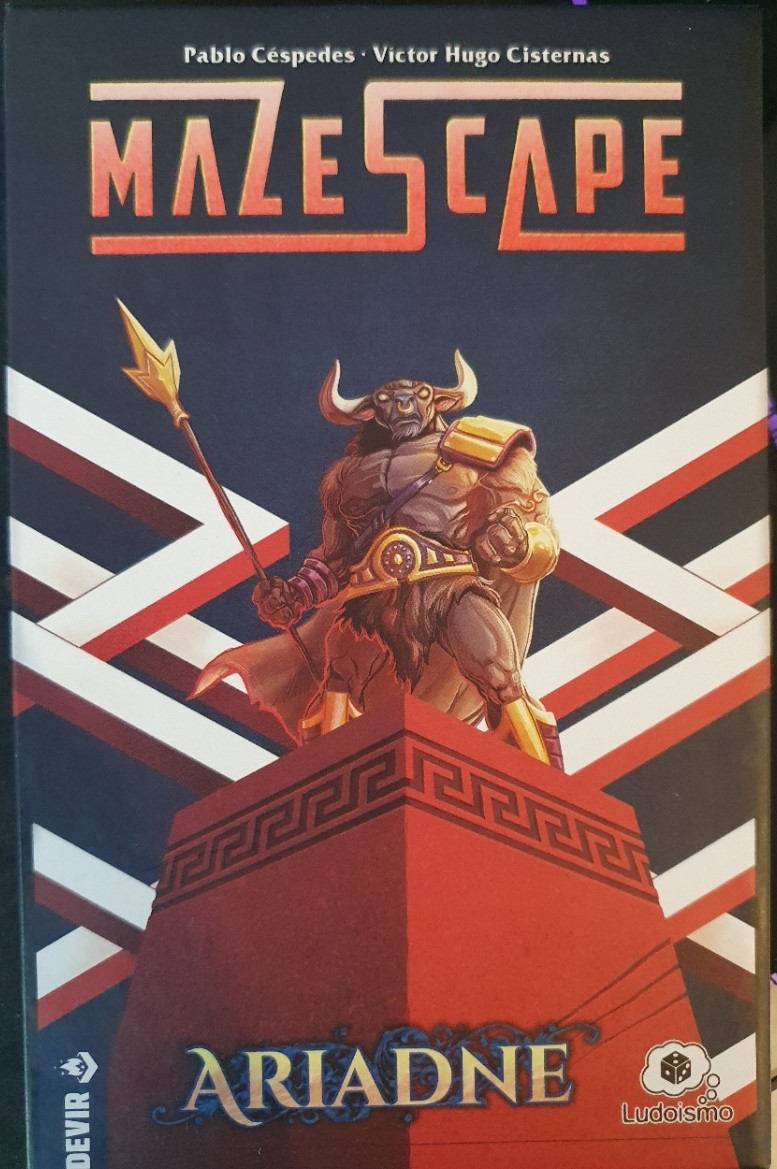
\includegraphics[width=1\linewidth]{content/pictures/MazeScape.jpg}
\caption{Verpackung des Spiels MazeScape (vgl. \cite{noauthor_mazescape_nodate})}
\label{fig:mazescape}
\end{figure}

\begin{figure}[ht]
\centering

\includegraphics[width=1\linewidth]{content/pictures/MazeScape_Level02.jpg}
\caption{Level 02 aus dem Spiel MazeScape (vgl. \cite{noauthor_mazescape_nodate})}
\label{fig:mazescape_level-02}
\end{figure}

% Der Vortest umfasste das Spielen eines Levels aus dem Spiel MazeScape (vgl. Abbildung \ref{fig:mazescape}). Die Regeln wurden für den Anwendungszweck abgeändert. Die Probanden mussten zu zweit die 
Der Vortest umfasste das Spielen des zweiten Levels (vgl. Abbildung \ref{fig:mazescape_level-02}) aus dem Spiel \say{MazeScape} (vgl. Abbildung \ref{fig:mazescape}). Die grundlegenden Regeln des Spiels bezüglich der Bewegung durch die Spielwelt wurden für diesen Anwendungszweck übernommen. Die weiteren Regeln den Spiels zu bestimmten Gegenständen, Punkten oder Gegnern wurden aus dem Grund der fehlenden Relevanz nicht berücksichtigt. Die Probanden hatten zehn Minuten Zeit um gemeinsam vom Startpunkt im Level an das Ziel zu kommen. Es war dabei nicht wichtig rechtzeitig ans Ziel zu kommen.

Dieser Vortest wurde gemacht, damit ein Grundwert der bestehenden Kommunikation zwischen den Probanden zu bestimmen. Dieser sollte sich nach dem Nachtest verbessert haben.

Nach erfolgreich oder nicht erfolgreichem Abschluss des Vortests durften die Probanden den Prototyp von Connecting-Minds testen. Sie erhielten zunächst eine Einführung zur Steuerung der jeweiligen Anwendung. Anschließend durften sie starten. Sie hatten hierfür 40 Minuten Zeit. Ziel war es, die Rätsel zu lösen, allerdings war es nicht wichtig, ob sie das Tutorial erfolgreich in der gegebenen Zeit abschließen.

Die Zuordnung welcher Proband welche Spielrolle einnimmt, wurde nach der Begrüßung der Probanden vollzogen. Für die ersten Fragebögen war es wichtig zu wissen, wer welche Rolle im Spiel einnimmt. Daher erfolgt zum Ausfüllen der Einverständniserklärung die Einteilung von den Probanden ausgehend.

Nach absolvieren des Prototyps mussten die Probanden die Fragebögen zu den Themen System Usability, Immersion, Spiel Erfahrung Motivation und dem Workload des jeweiligen Probanden ausfüllen.

Im Anschluss folgte nun der Nachtest. Hierfür mussten die Probanden erneut ein Level aus dem Spiel MazeScape spielen. Sie spielten dabei das Level 3 (vgl. Abbildung \ref{fig:mazescape_level-03}). Wie im Vortest wurden die gleichen Regeln zur Bewegung durch die Spielwelt für den Versuch angewandt. Alle anderen Regeln wurden ebenfalls nicht berücksichtigt. Die Schwierigkeit, die sich in diesem Level für die Probanden ergeben hat, ist dass sie dass Ziel zunächst zusammen suchen müssen ehe sie einen Weg durch das Labyrinth finden können.

\begin{figure}[ht]
\centering

\includegraphics[width=1\linewidth]{content/pictures/MazeScape_Level03.jpg}
\caption{Level 03 aus dem Spiel MazeScape (vgl. \cite{noauthor_mazescape_nodate})}
\label{fig:mazescape_level-02}
\end{figure}

Wie im Vortest hatten die Probanden hierfür ebenfalls zehn Minuten Zeit. Außerdem war es ebenso nicht wichtig das Ziel zu erreichen.

Nach Abschluss wurden die letzten Fragebögen von den Probanden ausgefüllt. Sie behandelten Vergleichswerte im Bezug auf die gegenseitige Beziehung und dem affektiven Status. Außerdem mussten sie Fragebögen zum Thema Leadership und dem Umgang mit Menschen in diesem Versuchsaufbau ausfüllen. Zuletzt hatten sie noch ein Freitextfeld, bei dem ihr qualitatives Feedback zur Anwendung gegeben werden konnte.

Nachdem alle Fragebögen ausgefüllt wurden, wurde die Aufnahme beendet und es wurde sich bei den Probanden für die Teilnahme bedankt. Sie durften sich noch etwas von den bereitgestellten Snacks nehmen und wurden im Anschluss entlassen.

Die gesamte Versuchsdurchführung dauerte etwa 75 Minuten pro Probanden-paar.

\subsection{Rahmenbedingungen}
Für die Durchführung des Versuchsaufbaus wurde im I Bau der ehemaligen Fakultät Digitale Medien der Seminarraum reserviert. 

Da für das Durchführen der Probandentests einiges an Hardware benötigt wurde, wurde diese bei der Fakultäts-\ac{IT} und dem \ac{IIIUS}. Über die \ac{IT} wurden der Rechner, Bildschirm, Tastatur und Maus ausgeliehen, über welchen der Player seine Anwendung spielen konnte. Über das \ac{IIIUS} wurde das Google Pixel 7, ein Stativ und die Aufnahme Kamera von Sony ausgeliehen. Über das Smartphone konnte der Watcher seine Anwendung spielen. Die Kamera und das Stativ wurden gebraucht, um die Versuchsdurchführung aufzunehmen. Außerdem wurde bei Herrn Prof. Dr. Schnell ein TP-Link Router ausgeliehen, da sich die Anwendung des Players und des Watchers innerhalb des gleichen Netzwerkes befinden müssen um sich mit dem Server zu verbinden. Das Netzwerk der Hochschule verbietet es, dass sich Geräte innerhalb des Netzwerkes finden können.
Auf einem privaten Laptop liefen der Docker-Container der MongoDB und der Node-Server über den der WebSocket Server erzeugt wird. Außerdem wurde ein Wimaxit 15-Zoll Touchmonitor verwendet, über den der Player seinen Avatar durch die Spielwelt steuern konnte.

\begin{figure}[ht]
\centering
\includegraphics[width=1\linewidth]{content/pictures/Aufbau_00.jpg}
\caption{Versuchsaufbau des Experiments}
\label{fig:study-experiment-00}
\end{figure}

\begin{figure}[ht]
\centering
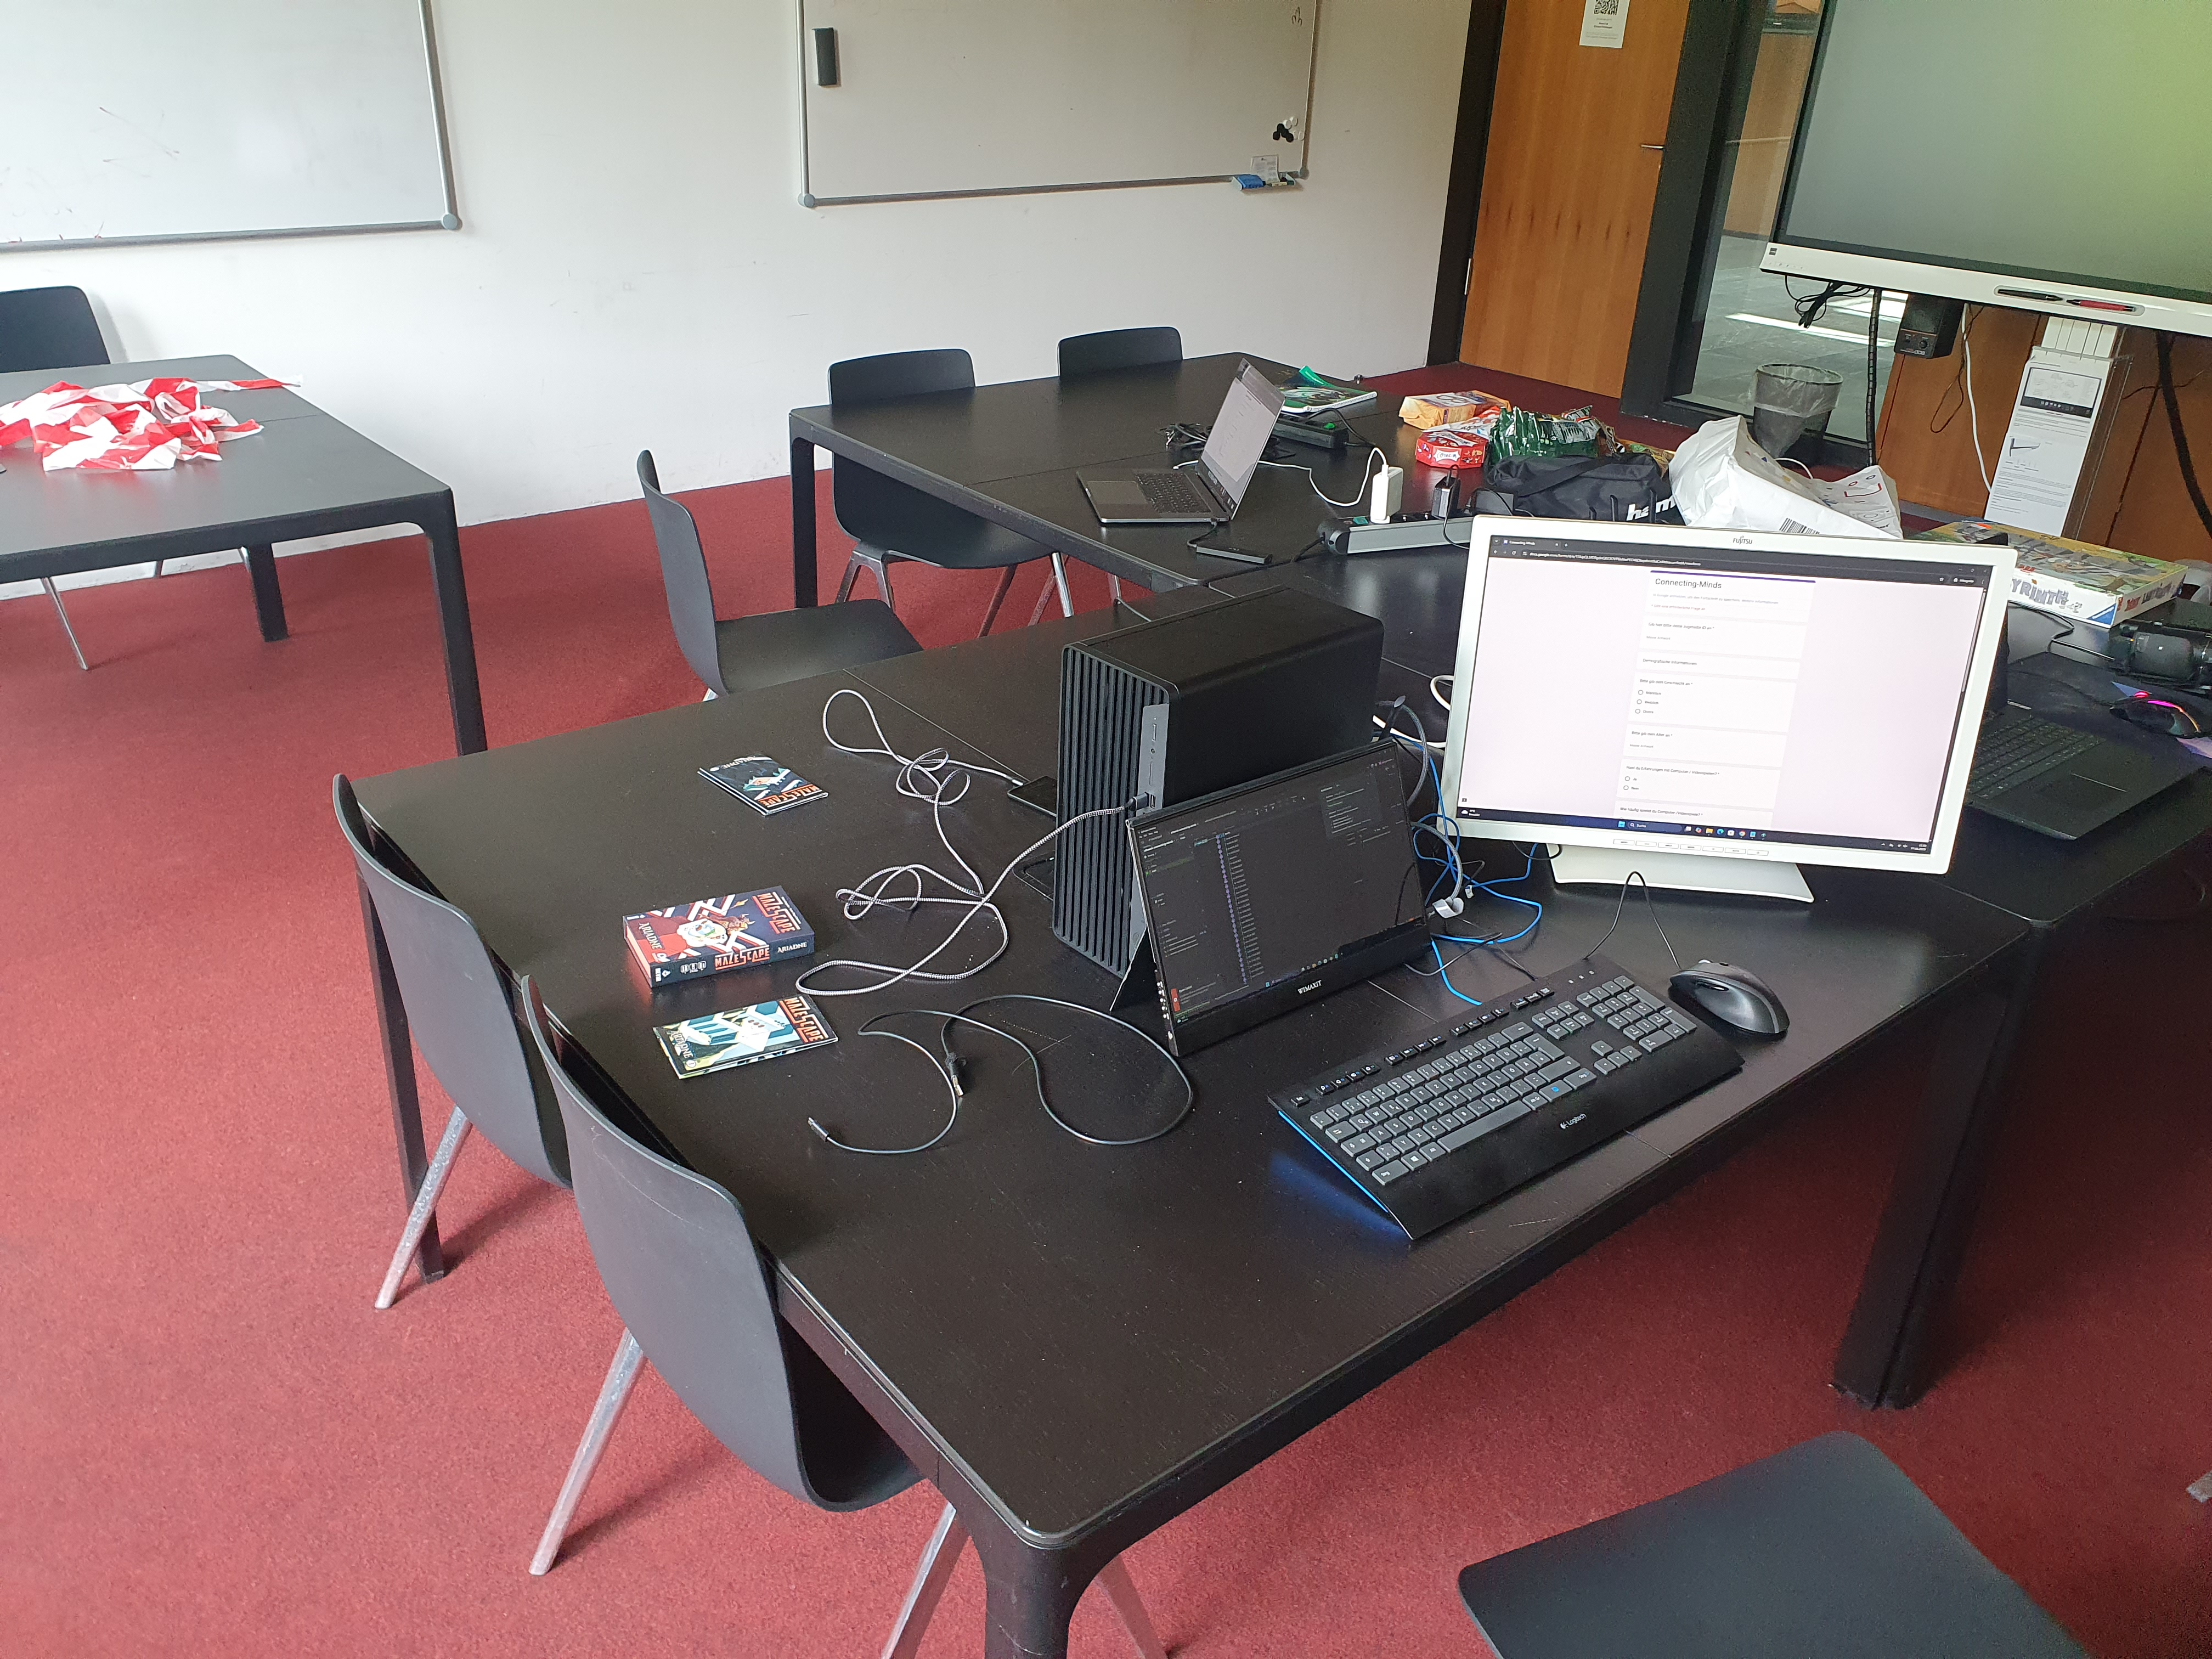
\includegraphics[width=1\linewidth]{content/pictures/Aufbau_01.jpg}
\caption{Versuchsaufbau Seite des Players}
\label{fig:study-experiment-01}
\end{figure}

\begin{figure}[ht]
\centering
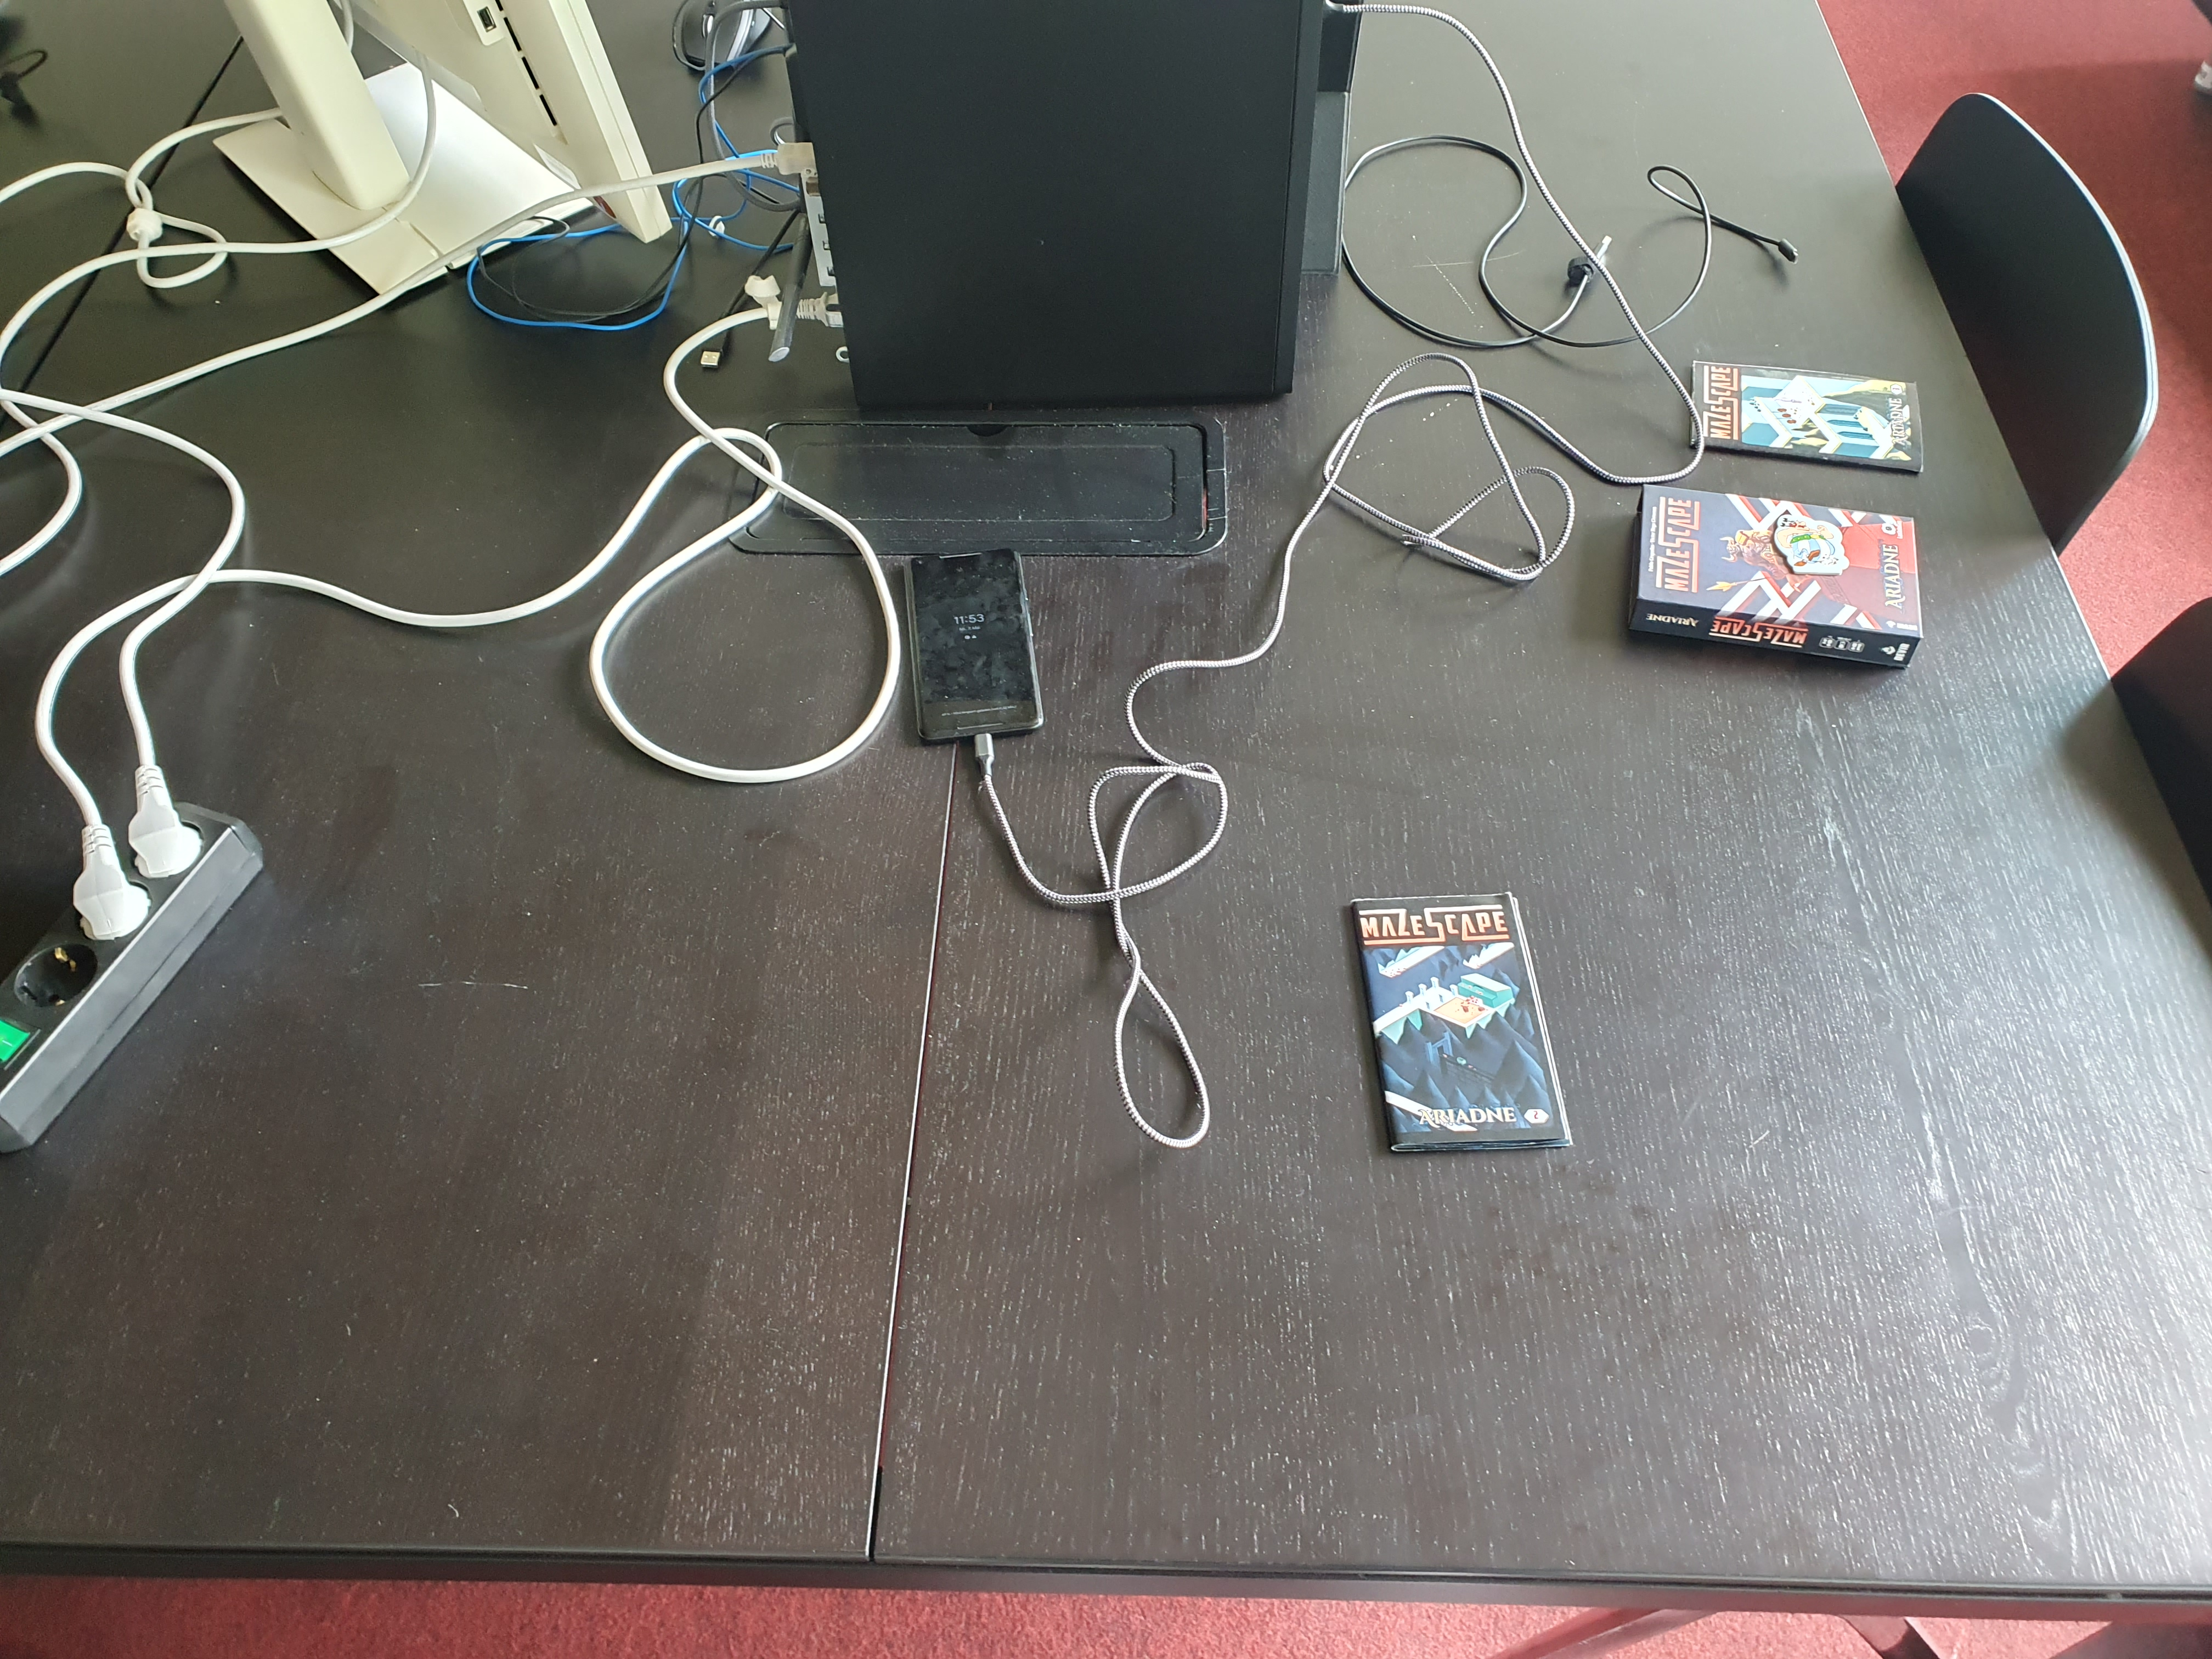
\includegraphics[width=1\linewidth]{content/pictures/Aufbau_02.jpg}
\caption{Versuchsaufbau Seite des Watchers}
\label{fig:study-experiment-02}
\end{figure}

Abbildung \ref{fig:study-experiment-00} zeigt wie der Seminarraum für die Versuchsdurchführung hergerichtet wurde. Beide Spielteilnehmer befinden sich jeweils gegenüber sitzend an einem quadratischen Tisch. Zwischen ihnen steht der Rechner der Player-Anwendung, damit sie physisch eine kleine Absperrung zwischen sich haben. Diese Absperrung ist grundlegend nicht relevant gewesen. So sollte vermieden werden, dass sich die beiden -Versuchsteilnehmer in die Anwendung des anderen schauen und so ggf. ohne den Einsatz der Kommunikation eine Lösung gefunden wird. Es war ihnen verboten in die Anwendung des anderen zu schauen.

Auf der rechten Seite des Tisches saß der Player (vgl. Abbildung \ref{fig:study-experiment-01}), der über den vor sich stehenden Touchmonitor seine Anwendung spielen konnte. Über den großen Bildschirm sollte er die Fragebögen der Versuchsdurchführung ausfüllen. Hierzu bekam der eine Tastatur und Maus. Der Watcher saß an der linken Seite des Tisches (vgl. Abbildung \ref{fig:study-experiment-02}). Hier konnte der Watcher über das beigelegte Google Pixel die Anwendung des Watchers spielen. Gespielt wurde die fertig gestellte \ac{3D}-Anwenung des Watchers. Außerdem sollten auf dieser Seite des Tisches die Probanden den Vor- und Nachtest des Versuches spielen. Dazu konnten sie sich entweder auf die Stühle setzen und durch das Labyrinth navigieren oder sie stellten sich hin.

Am hinteren linken Bildrand von Abbildung \ref{fig:study-experiment-00} steht ein weiterer Laptop, über welchen der Watcher seine Fragebögen ausfüllen musste.

\section{Ergebnisse}
In diesem Abschnitt werden die Ergebnisse der verschiedenen Fragebögen und der Aufzeichnungen der Versuchsdurchführungen vorgestellt.
Die Vorstellung erfolgt in drei Abschnitten. Zunächst werden die Ergebnisse der Demographischen Daten vorgestellt, im Anschluss erfolgt die Vorstellung der Ergebnisse bezüglich des Prototyps und zum Schluss werden die Kenntnisse aus den Aufnahmen vorgestellt.

\subsection{Vorstellung der demographischen Daten}
An der Versuchsdurchführung haben N=14 freiwillige Probanden (3 weibliche und 11 männliche; M = 25,86; SD = 4,52 Jahre) teilgenommen. Daraus ergeben sich für die Versuchsdurchführung 7-Zweierpaare. Zwei Probanden kannten sich zum Start der Versuchsdurchführung nicht, bzw. kannten sich nur vom Sehen. 12 der Probanden haben angegeben, dass sie bereits Erfahrungen mit Video- und Computerspielen gemacht haben, zwei hingeben haben bislang keine Erfahrungen gesammelt (fünf spielen mehr als 10 Stunden pro Woche, drei 6-10 Stunden, jeweils zwei spielen 3-5 und 1-2 Stunden pro Woche und zwei 0 Stunden die Woche. 13 von ihnen haben angegeben, dass sie bereits Erfahrungen mit Multiplayer-Spielen gesammelt haben, eine Person nicht (drei von ihnen spielen mehr als 10 Stunden Multiplayer-Spiele, einer 6-10 Stunden, vier 3-5 Stunden, fünf 1-2 Stunden und wieder eine Person 0 Stunden in der Woche). Insgesamt spielen 11 der Probanden kompetitive Multiplayer-Spiele, 10 kooperative, fünf kollaborative und eine Person andere Arten.
Auf die Frage nach Vorerfahrungen mit Spielen, die über eine Touchsteuerung gespielt werden, haben 13 \say{Ja} angeben, eine Person nein (eine Person spielt oft Spiele mit Touchsteuerung, drei Personen manchmal und  10 selten).

Die Abfrage bezüglich des Spielertyps ergab, dass sich sieben Teilnehmer des Typs Explorer, vier Teilnehmer des Typs Achiever, drei des Typs Killer und keiner des Typs Socializer zugehörig empfanden.

\subsection{Vorstellung der Prototyp-Evaluation}
Die Vorstellung der Fragebögen wird in die Dimensionen quantitative und qualitative Ergebnisse unterteilt.

In der quantitativen Auswertung der Fragebögen \ac{SUS}, \ac{GEQ}, \ac{IMI} und \ac{NASA-TLX} wurden zunächst für jeden Fragebogen bzw. dessen Subkategorien der \ac{M} und die \ac{SD} berechnet. Diese deskriptiven Kennwerte wurden für die Gesamtstichprobe (n = 14) sowie getrennt für die Gruppen \textit{Player} und \textit{Watcher} bestimmt, um mögliche Unterschiede zwischen den beiden Anwendungen zu identifizieren.

Zur Überprüfung signifikanter Gruppenunterschiede wurden die Daten in einem ersten Schritt auf Normalverteilung geprüft. Diese Prüfung erfolgte sowohl visuell anhand von \ac{Q-Q}-Diagrammen als auch mithilfe des Shapiro-Wilk-Tests. Diese Tests wurden jeweils separat für die Gruppen Player und Watcher durchgeführt. 

Je nach Ergebnis der Normalitätsprüfung kam für den anschließenden Gruppenvergleich ein unterschiedliches statistisches Verfahren zum Einsatz: Bei vorliegender Normalverteilung in beiden Gruppen wurde ein zweiseitiger t-Test für unabhängige Stichproben verwendet. Wenn mindestens eine Gruppe keine Normalverteilung aufwies, wurde stattdessen der Mann-Whitney-U-Test als nichtparametrische Alternative herangezogen.

Der folgende Abschnitt stellt nun die Ergebnisse dieser Auswertung für die einzelnen Fragebögen im Detail dar.
\paragraph{Quantitative Ergebnisse}
Der \ac{SUS} (Wertung zwischen 1: \say{stimme überhaupt nicht zu} und 5: \say{stimme voll und ganz zu}) ergab eine marginal hohe Usability (M = 69,11; SD = 13,64), wobei es starke Ausschläge nach oben (max = 92.5) und unten (min = 47.5) gibt. Damit eine Anwendung eine gute Usability haben kann muss sie mindestens einen Score von 73 haben (vgl. \cite[S. 36]{brooke_sus_2013}). In Bezug auf Unterschiede der Usability zwischen der Anwendungen des Watchers (M = 68,93; SD = 14,28) und des Players (M = 69,29; SD = 14,12) konnte über den t-Test (p = 0,95; t = 2,29) kein signifikanter Unterschied festgestellt werden.

Die Mittelwerte der einzelnen Kategorien des InGame Moduls des \ac{GEQ}s (Wertung zwischen 0: \say{überhaupt nicht} und 4: \say{extrem}) zeigen, dass die Probanden Spaß beim Spielen der Anwendungen hatten (Positive Emotionen: M = 3,07; SD = 0,83; Negative Emotionen: M = 0,54; SD = 0,75). Die Werte des Flows ( M = 3; SD = 0,94), Kompetenz (M = 2,54; SD = 0,89), Immersion (M = 2,54; SD = 0,89) und Herausforderung (M = 2,32; SD = 0,58) unterstützen dies, auch wenn sie nicht ganz so hoch bewertet wurden. Zwischen der Player und Watcher Anwendung beweisen der t-Test für Kompetenz (p = 0,19; t = 2,18), Flow (p = 0,42; t = 2,21) und Immersion (p = 0,60; t = 2,24) sowie der Mann-Whitney-U-Test für die restlichen Dimensionen keine signifikanten Unterschiede in den Bewertungen der einzelnen Komponenten (Anspannung: p = 0,65; U = 20,5; Herausforderung: p = 0,33; U = 17; negative Emotionen: p = 0,84; U = 22,5; positive Emotionen: p = 0,6; U = 20).

Die Mittelwerte des sozialen Präsenz Abschnittes des \ac{GEQ}s (Wertung zwischen 0: \say{überhaupt nicht} und 4: \say{extrem}) zeigen, dass die Teilnehmer gegenseitig Empathie verspürt (M = 3,11, SD = 0,55), wenig negative Gefühle gezeigt (M = 1,26; SD = 0,57) und verhaltensbezogene Beteiligung (M = 3,36; SD = 0,56) gezeigt haben. Auch hier gibt es keine Unterschiede in der Bewertung von Player und Watcher (Empathie: p = 0,855; U = 22.5; Negative Gefühle: p = 0,14; t = 2,19; Beteiligung: p = 0,45; t = 2,18).

Die Mittelwerte des Post-Game-Modul des \ac{GEQ}s (Wertung zwischen 0: \say{überhaupt nicht} und 4: \say{extrem}) zeigen, dass positive Erfahrungen (M = 2,38; SD = 0,88), wenn auch nicht so stark, aus dem Prototyp überbleiben, jedoch die Rückkehr in die Realität (M = 1,02; SD = 0,69) leicht fiel. Geringe Negative Erfahrungen (M = 0,31; SD = 0,31) zeigen, dass der durch die Usability entstandene Frust nicht überbleibt und die Probanden nicht ermüdet wurden (M = 0,68; SD = 0,82). In den Einzelkategorien der Positiven Erfahrungen (p = 0,56; t = 2.18), Negative Erfahrungen (p = 0,3: U = 16) und Müdigkeit (p = 0,88; t = 2,18) existiert kein signifikanter Unterschied zwischen den Anwendungen. Hingegen hat die Kategorie Rückkehr in die Realität (p = 0,04; U = 8.5) einen signifikanten Unterschied zwischen der Anwendung des Players und des Watchers. Der Mittelwert (M) der Watcher Anwendung wurde mit 1,43 höher bewertet als die des Players (0,62). Dieser Wert ist nicht hoch, allerdings hat die Anwendung des Watchers, vermutlich aufgrund ihrer Funktionen und der Führungsrolle im Design eine andere Wirkung, als die des Players.

Das Ergebnis des Abschnittes Interesse/ Vergnügen zeigt des \ac{IMI} (Wertung zwischen 1: \say{trifft überhaupt nicht zu} und 5: \say{trifft völlig zu}) zeigen, dass die Probanden überwiegend Interesse und Vergnügend zeigen konnten (M = 3,60; SD = 1,38). Zwischen der Bewertungen der Player und Watcher konnte kein signifikanter Unterschied festgestellt werden (p = 0,45; t = 2,21). 

Der \ac{NASA-TLX} zeigt (Basis Skala von 0 bis 10; skaliert auf 100er Skala), dass die Rätsel und die Steuerung eine höhere geistige Anstrengung (M = 63,57; SD = 14,47), eine sehr geringe körperliche Belastung (M = 4,29; SD = 6,46) und eine geringe zeitlich Anstrengung (M = 28,57; SD = 16,57) fordert. 
Der Prototyp konnte durchweg erfolgreich abgeschnitten werden, das zeigt der Leistungsteil (M = 75,14; SD = 17,85) des Fragebogens. Außerdem bot er eine durchwachsene Anstrengung (M = 50,71; SD = 19,79) und geringe Frustration (M = 29,29; SD = 31). Die umgesetzten Rätsel waren in ihrer Schwierigkeit nicht zu schwierig, boten allerdings dennoch eine Herausforderung. Die verbesserungswürdige Usability zeigt sich hier jedoch in der Frustration erneut. Zwischen der Anwendung des Players und Watchers konnten in den Unterkategorien (Geistige Anforderungen: p = 0,86; t = 2,22; Körperliche Anforderungen: p = 0,55; U = 29; Zeitliche Anforderungen: p = 0,76; t = 2,23; Leistung: p = 0,78; t = 2,21; Anstrengung: p = 0,9; t = 2,19; Frustration: p = 0,85; U: 26,5) keine signifikanten Unterschiede festgestellt werden.


Für die qualitative Auswertung des Freitextfeldes \say{Welches sonstige Feedback hast du?} aus dem allgemeinen Feedback zur Nutzerstudie und des Prototyps wurde sich an der thematischen Analyse von \cite{braun_using_2006} orientiert. Dabei wurde der sechs-stufige Prozess angewandt: Zunächst wird sich mit den Daten vertraut gemacht, danach werden erste Kategorien erstellt. Im Anschluss werden einzelne Themen gesucht, darauffolgend werden die Themen kontrolliert. Danach werden Themen definiert und benannt. Zum Schluss wird das Ergebnis präsentiert.

\paragraph{Qualitative Ergebnisse}
Abbildung \ref{fig:qualitative-results} zeigt, dass die Antworten aus dem Freitextfeld des Fragebogens in fünf Kategorien unterteilt werden können.
Unterteilt können die Ergebnisse in konstruktiver Kritik bezüglich der Anwendungen und allgemeinem positiven Feedback zum Spielkonzept und der Studie.
% Die Hauptthemen dabei sind die mangelhafte Steuerung, hauptsächlich die des Watchers, der Anwendungen 
Das Hauptthema der konstruktiven Kritik umfasst die verbesserungswürdige Steuerung, hauptsächlich die des Watchers, der Anwendungen. Zusammengefasst wurden jedoch das Rätsel und Environment-Design ebenfalls erwähnt.

% Im Kern wurde bei der Steuerung bemängelt, dass die manchmal umständlich, unintuitiv und unresponsiv ist. Weitere Aussagen beziehen sich dabei auf die Dreh- und Zoom Gesten der Watcher-Anwendung. Zudem wird vorgeschlagen diese in zwei Schritte aufzuteilen, damit sich diese nicht zu sehr überlagert. Vorgeschlagen wurde ebenfalls diese durch On-Screen Overlays zu ergänzen, um eine Unterteilung zwischen Zoom und Yaw zu erzielen. In Bezug auf die Steuerung des Players wurde darauf hingewiesen, dass die Veränderung der Sichtweise nach oben und unten in der First-Person-Ansicht nicht möglich und somit nur ein eingeschränktes Blickfeld vorhanden war. Außerdem gab es Schwierigkeiten in der Bewegung des Avatars, da teilweise kein Ziel ausgewählt werden konnte. 

\begin{figure}[ht]
\centering
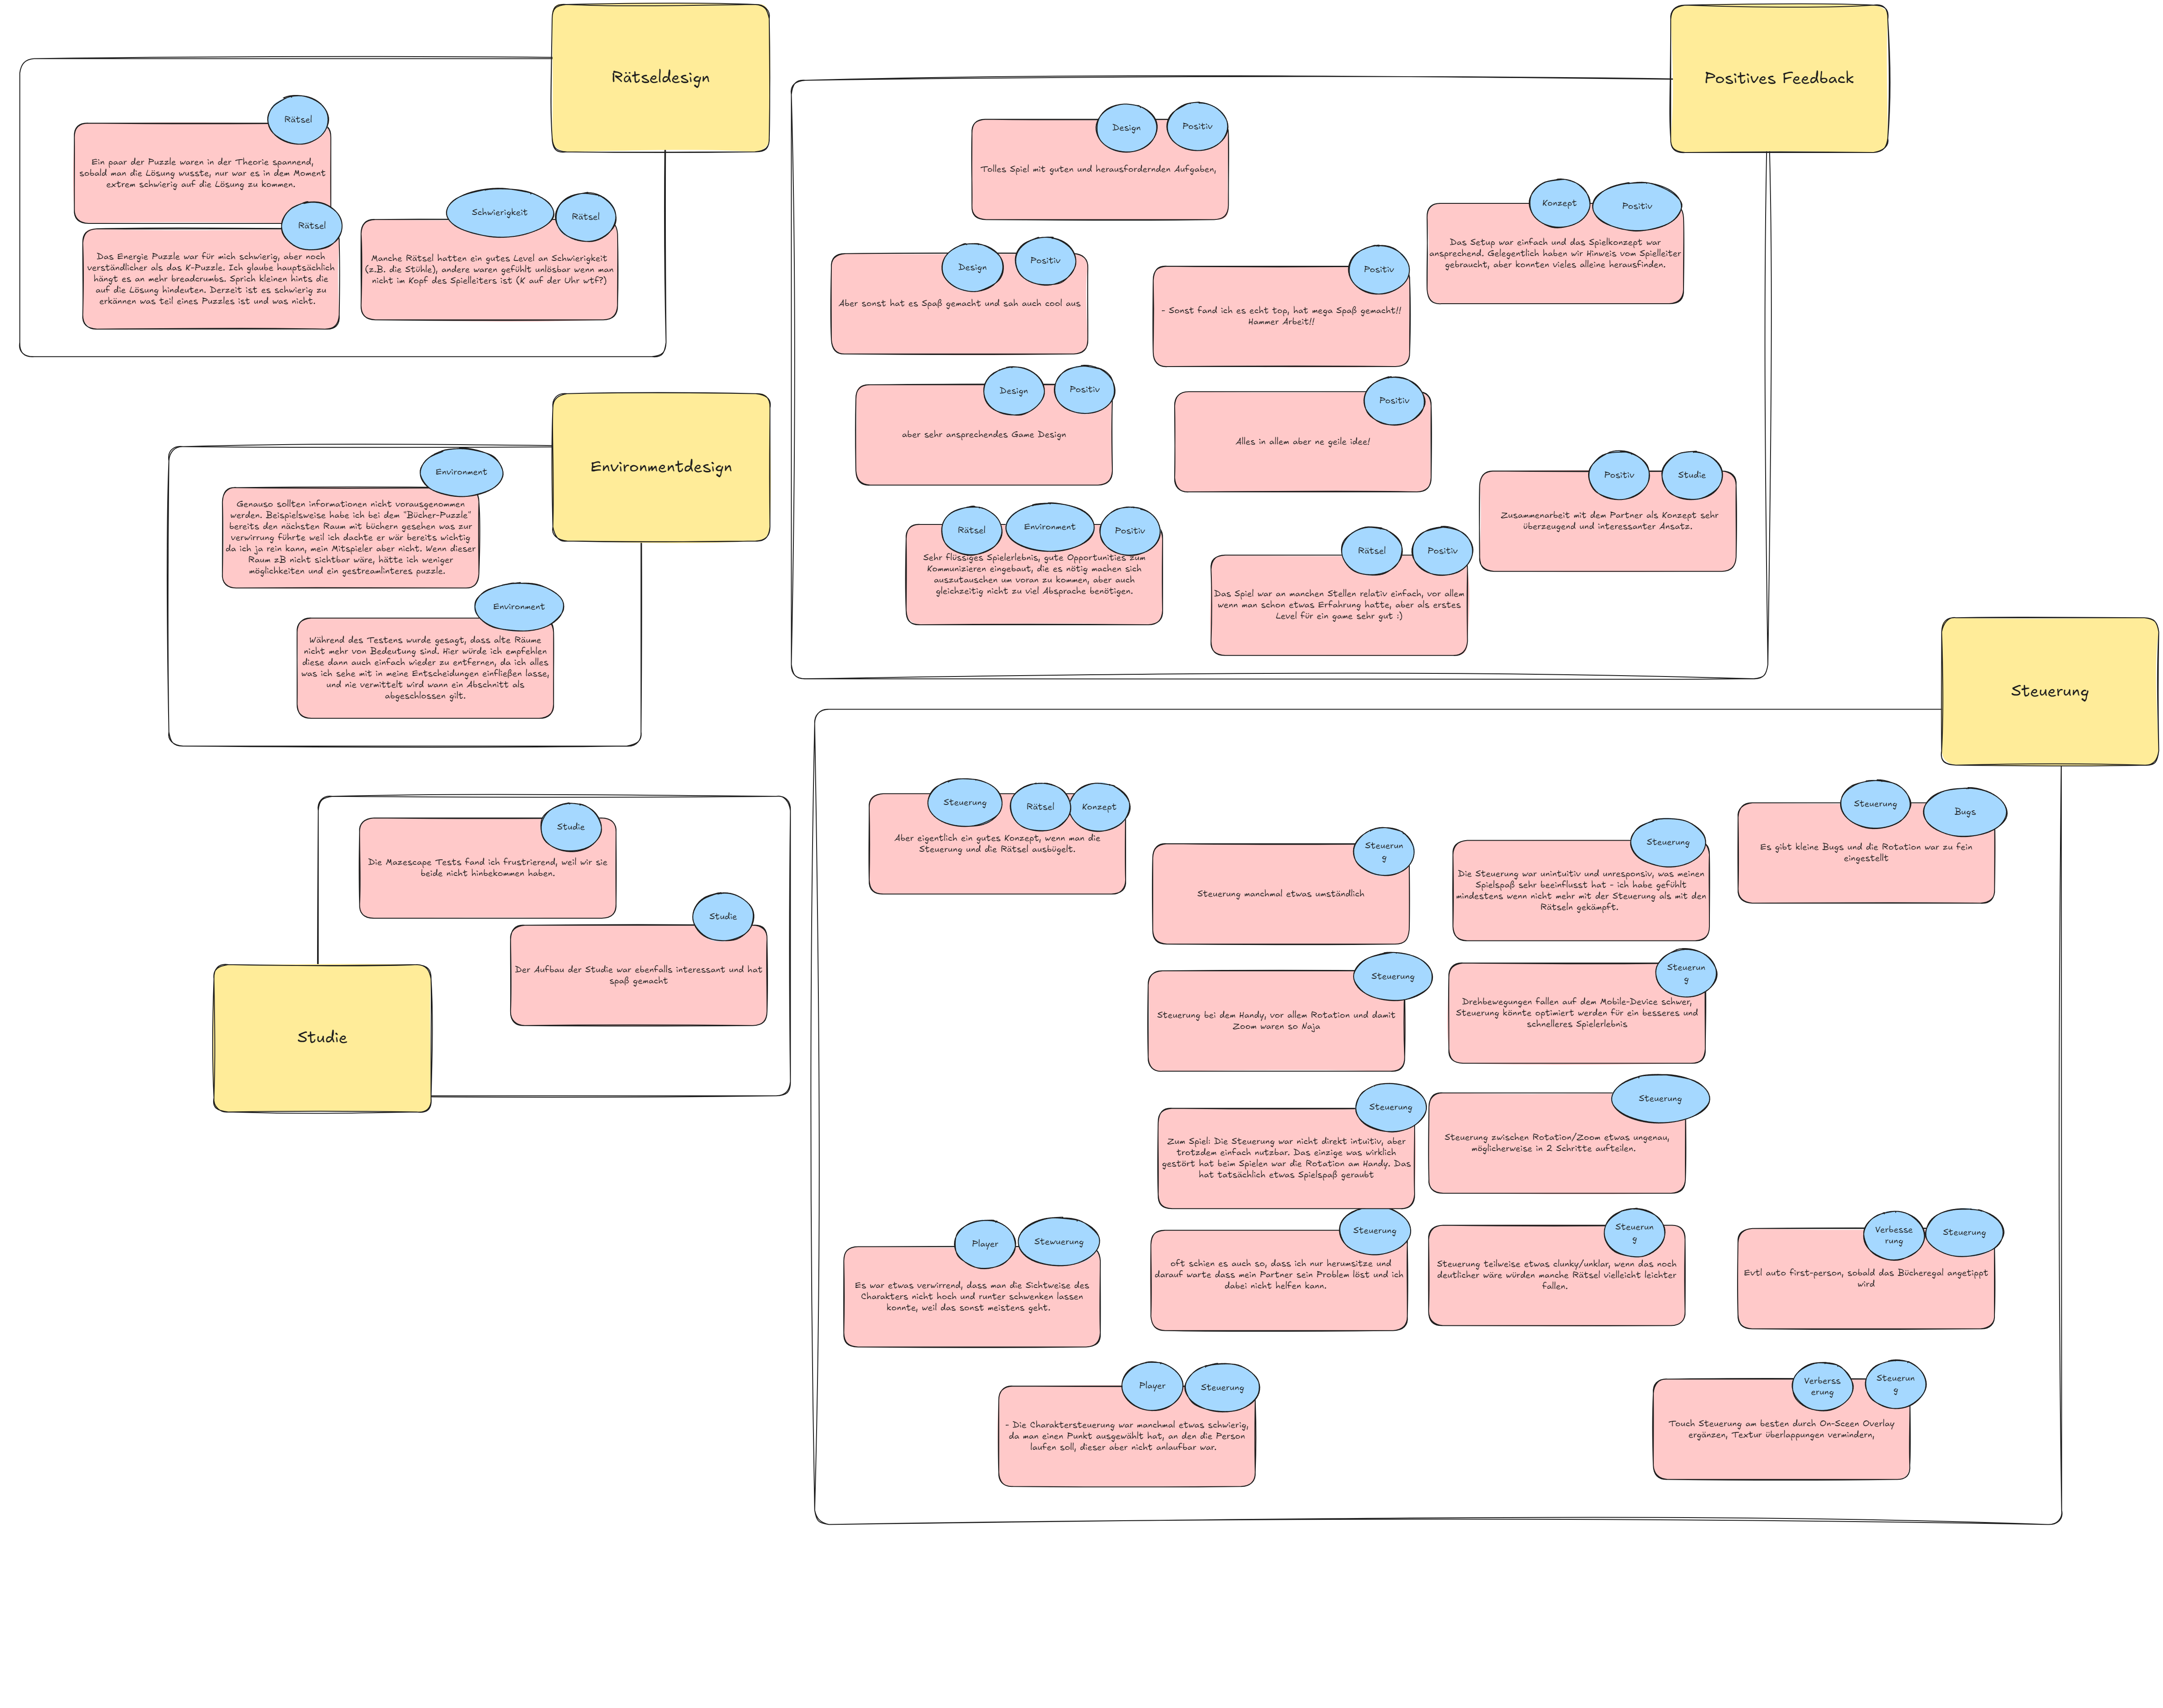
\includegraphics[width=1\linewidth]{content/pictures/Qualitative-Auswertung-Schritt-1.png}
\caption{Ergebnis der groben Kategorisierung nach \cite{braun_using_2006}}
\label{fig:qualitative-results}
\end{figure}

Abbildung \ref{fig:qualitative-results-end} zeigt die Zusammenführung des Feedbacks. 
Die Steuerung, vor allem die des Watchers, wird insgesamt als problematisch wahrgenommen. Mehrere Rückmeldungen beschreiben sie als umständlich, unintuitiv, unresponsiv oder \say{clunky} und unklar. Betroffen sind hierbei die Yaw- und Zoom - Geste der \ac{3D}-Anwendung. Mögliche Verbesserungsvorschläge, die benannt wurden, handelten von unterstützenden Elementen im Overlay-\ac{UI} des Spielers. So könnte eine bessere Unterscheidung zwischen dem Zoomen und dem Rotieren der Ansicht geschaffen werden. 
In der Player-Anwendung wurde das Fehlen einer vertikalen Bewegung der Kamera in der First-Person-Ansicht bemängelt, da momentan die Ansicht nur von einer vertikalen Perspektive aus genutzt werden kann. Zusätzlich gab es öfters Probleme damit, eine Zielposition auszuwählen, an die sich der Avatar bewegen soll.

In Bezug auf das Rätsel/ und Umgebungsdesign wurde bemängelt, dass teilweise die Lösungsfindung der Rätsel noch zu unausgereift und herausfordernd ist. 
Außerdem wird vorgeschlagen noch mehr Hinweise auf die Rätsel einzubauen, damit die Lösungsfindung einfacher gestaltet werden kann. Zudem wurde bemängelt, dass die Anzahl der aktiven Räume nach dem Lösen wieder deaktiviert werden können, damit diese das Lösen der neuen Rätsel nicht mehr behindern.

Die Nutzerstudio wurde als interessant und gut gemacht empfunden, allerdings bot der Vor- und Nachtest mit MazeScape Frustrationsgefahr.

Alles in allem bot der Prototyp Spaß am Spielen. Außerdem wurde das Spielkonzept von \say{Connecting-Minds} als ansprechend und überzeugend Umgesetzt angesehen. Gelobt wurde zudem das einfach Setup.
\begin{figure}[ht]
\centering
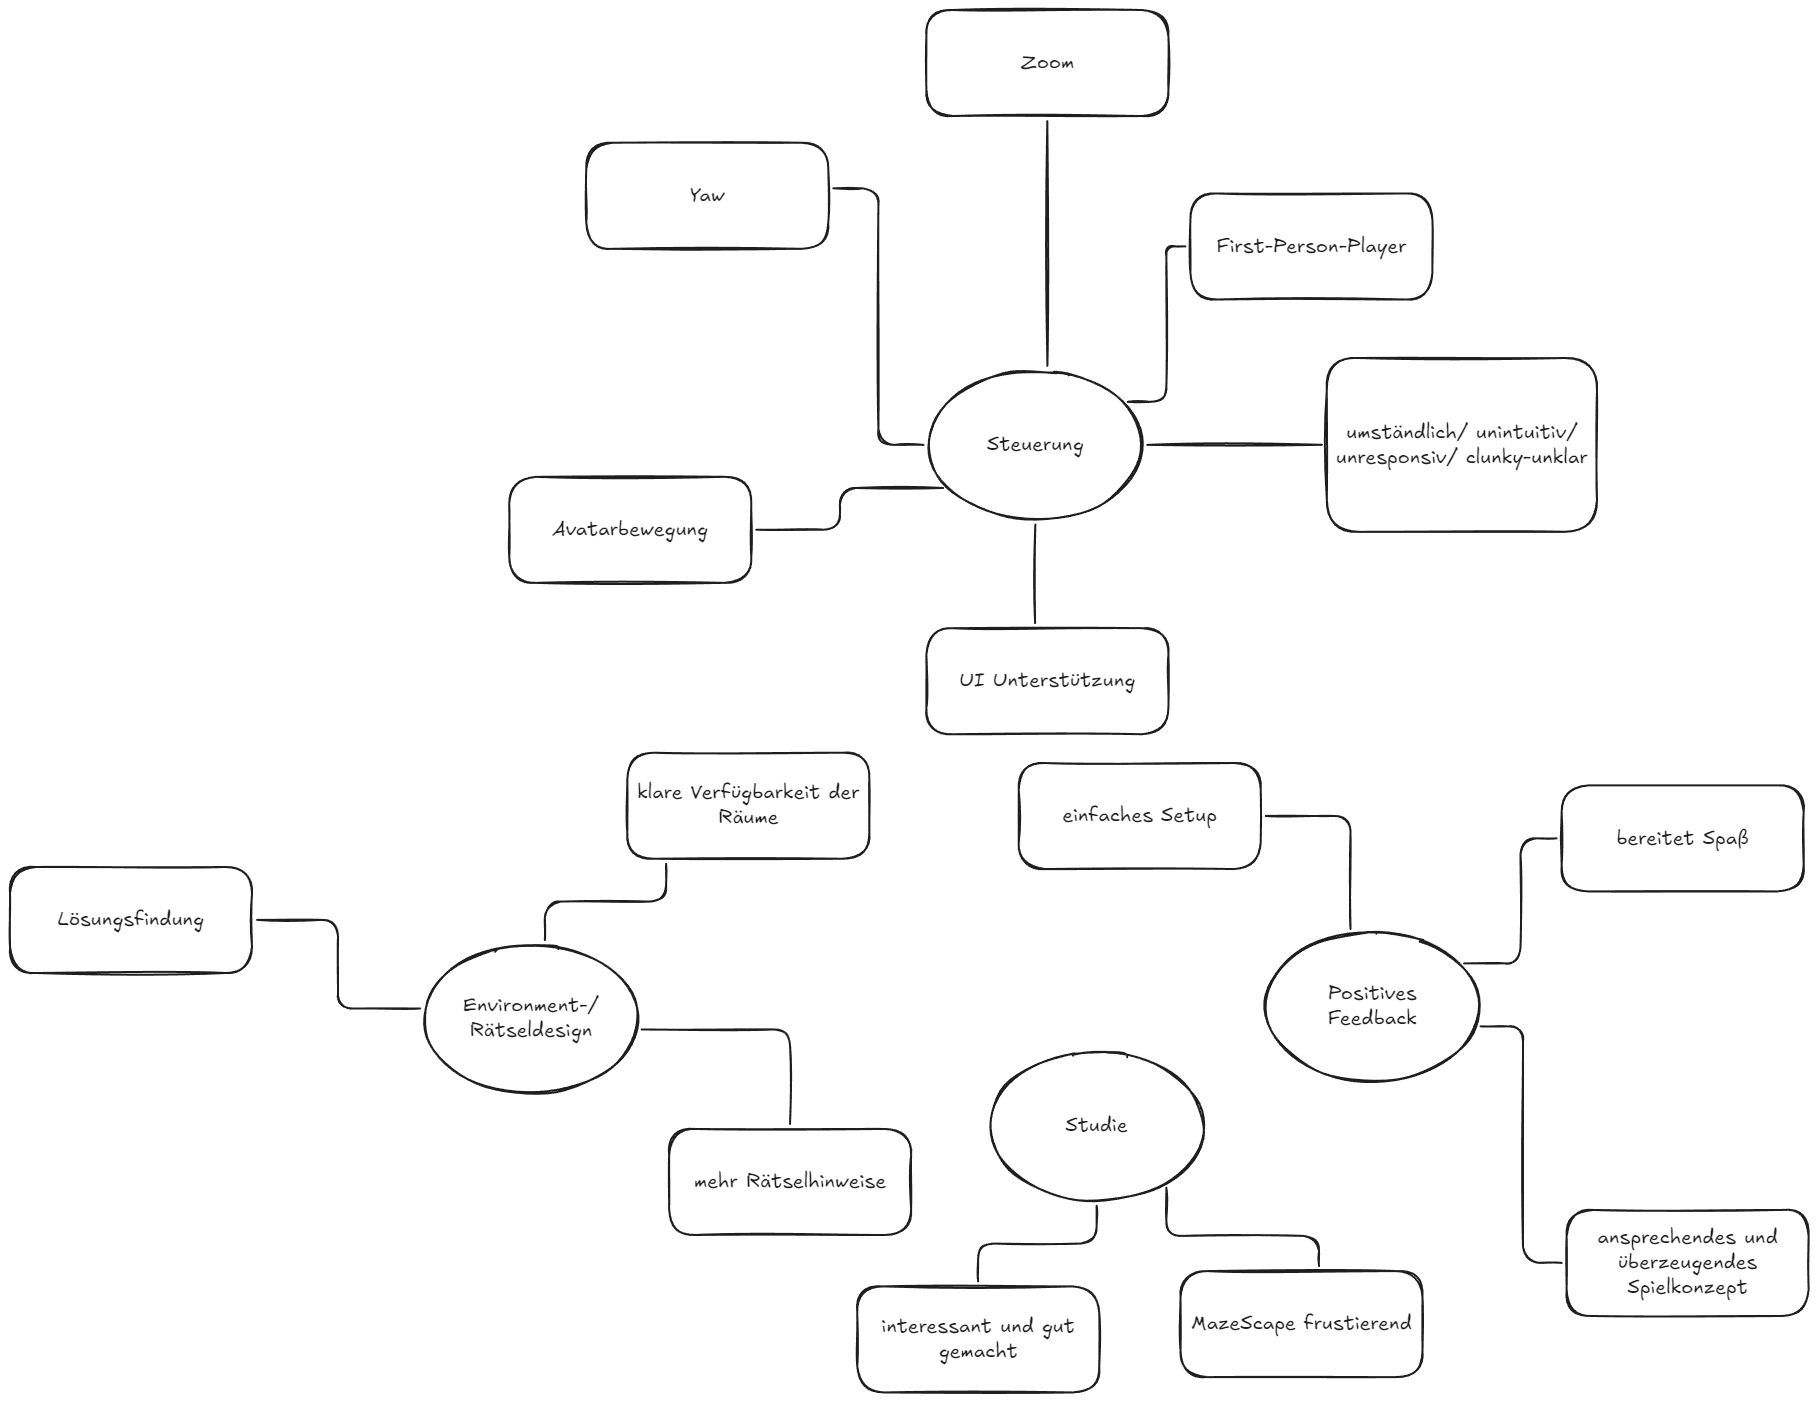
\includegraphics[width=1\linewidth]{content/pictures/Qualitative-Auswertung-Schritt-2.png}
\caption{Ergebnis der feinen Kategorisierung nach \cite{braun_using_2006}}
\label{fig:qualitative-results-end}
\end{figure}

% \paragraph{}

\subsection{Einordnung der qualitativen und quantitativen Ergebnisse}
Die Auswertung des Freitextfeldes zeigt genauere Ursachen bezüglich des niedrigen Wertes des \ac{SUS}'. Die niedrige Gebrauchstauglichkeit der  resultiert aus der fehlenden \say{Klarheit} und Verbesserungswürdigen Umsetzung der Steuerung der Anwendung des Watchers und des Players. Außerdem werden hier ebenfalls die angesprochenen Mängel des Rätsel- und Environmental-Designs berücksichtigt. Der allgemeine Durchschnitt der Frust-Skala aus dem \ac{NASA-TLX} kann hierbei nur bedingt als Unterstützung dienen. Der Mittelwert ist mit 29,29 nicht hoch, allerdings zeigt die Standabweichung von 31, dass bei einzelnen Probanden Frust erzeugt wurde. 

Die Ergebnisse des \ac{IMI}s und des \ac{GEQ}s zeigen, unterstützend durch das positive Feedback aus dem Freitextfeld, dass die Probanden trotz der genannten Schwierigkeiten Spaß und Freude entwickeln konnten.

\subsection{Vorstellung der Ergebnisse der subjektiven Wahrnehmung der Probanden}
% Die Wahrnehmung des \ac{IOS} und \ac{SAM}s wurden sowohl vor dem Vortest also auch nach dem Nachtest gemessen. Sie sollen
Im Folgenden werden die Ergebnisse zur subjektiven Wahrnehmung der Probanden im Hinblick auf den \ac{IOS} und den \ac{SAM} dargestellt. Die Einschätzungen wurden zu zwei Zeitpunkten erhoben; einmal vor dem Vortest als \say{Ground-Truth} und einmal nach dem Nachtest, um mögliche Veränderungen im Erleben sozialer Nähe und Affektivität im Verlauf des Experiments sichtbar zu machen.

\begin{figure}[ht]
\centering
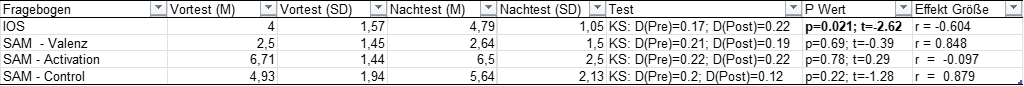
\includegraphics[width=1\linewidth]{content/pictures/IOS_SAM_Overal.png}
\caption{Ergebnisse des \ac{IOS} und \ac{SAM} auf alle Probanden bezogen}
\label{fig:ios_sam_overal}
\end{figure}

Abbildung \ref{fig:ios_sam_overal} zeigt die Ergebnisse des \ac{IOS}' und \ac{SAM}s. Der analysierte Datensatz umfasst sowohl die Antworten der Player als auch der Watcher. Eine Unterscheidung der Entwicklung in den einzelnen Rollen erfolgt im zweiten Schritt.

Zunächst wurden die Datensätze (der gesamte und seine Untergruppen) auf eine Normalverteilung überprüft. Dies erfolgte im gesamten Datensatz über den  Kolmogorov-Smirnov-Test (vgl. \cite{massey_kolmogorov-smirnov_1951}). Für die geteilten Datensätze wurden wie bei den Fragebögen zum Prototyp visuelle \ac{Q-Q}-Diagramme angelegt und anschließend über den Shapiro-Wilk-Test auf eine Normalverteilung validiert.

Insofern die Datensätze vom Vor- und Nachtest in Normalverteilung vorlagen, wurde der t-Test für abhängige Stichproben durchgeführt, um zu bestimmen ob die vorliegende Änderung signifikant ist. Außerdem wurde die Effekt Stärke der Datensätze bestimmt. Für nicht-parametrische Datensätze wurde der Wilcoxon-Test angewandt.

Zusätzlich wurden die Untergruppen auf den Vergleich der Veränderungen untersucht, um feststellen zu können, welche Untergruppe eine stärkere Entwicklung vorlegen konnte. Für parametrisierte Untergruppen wurde der Welch-Test angewandt, für nicht-parametrisierte der Mann-Whitney-U-Test.

\paragraph{Allgemeine Auswertung}

Zunächst ist zu beobachten, dass die empfundene Nähe der jeweiligen Probanden-Paare, die über den \ac{IOS} gemessen wurde, im Mittelwert ansteigt. Dies ist eine signifikante Veränderung, die belegt, dass sich die Probanden innerhalb des Versuchsaufbaus besser kennenlernen konnte und der Prototyp dabei ebenfalls eine Rolle gespielt hat. Es zeigte sich 

Die Valenz, also das Empfinden von positiver oder negativer Emotionen, (Wertung von 1 = glücklich bis 9 = unglücklich) stieg leicht an. Dies kann durch Frustration in den jeweiligen Vor- und Nachtests oder der Usability des Prototyps verursacht worden sein. Die Änderung der Valenz ist jedoch nicht signifikant. Die Activation bzw. die Anspannung (Wertung von 1 = aufgeregt bis 9 = entspannt) der Teilnehmer stieg ebenfalls leicht an. Diese Änderung ist ebenfalls nicht signifikant. Die entstandene Anspannung der Probanden kann durch die zeitlichen Begrenzungen, in welchen sie den Prototyp und die Vergleichstest durchführen müssen erklärt werden. Außerdem kann der zuvor erlittene Erfolg oder Frust über das Lösen oder nicht Lösens des Nachtests ebenfalls eine Rolle spielen. Der Abschnitt des Controls, der Dominanz der Probanden, (Wertung von 1 = kontrolliert bis 9 = in Kontrolle) steigt ebenfalls an. Allerdings ist dies ebenfalls keine signifikante Änderung. Die Wachsende Dominanz kann man dem wachsendem Selbstvertrauen, das die einzelnen Probanden im Verlauf des Experiments entwickeln konnten, zusammenhängen. Die Probanden lernen sich besser kennen und versuchen durch die Herausforderung der Vergleichstest das Ziel zu erreichen.

\paragraph{Auswertung in der Unterscheidung zwischen Player und Watcher}

\begin{figure}[ht]
\centering
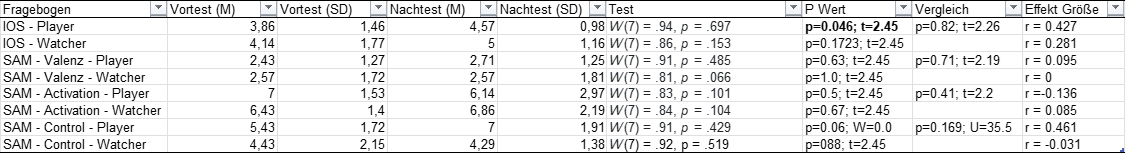
\includegraphics[width=1\linewidth]{content/pictures/IOS_SAM_Player_Watcher.png}
\caption{Ergebnisse des \ac{IOS} und \ac{SAM} auf beide Spielerrollen bezogen}
\label{fig:ios_sam_roles}
\end{figure}

Abbildung \ref{fig:ios_sam_roles} zeigt die Ergebnisse des \ac{IOS}' und \ac{SAM}s. Hierbei wurden nun der gesamte Datensatz in seine zwei Untergruppen, Player und Watcher, geteilt und getrennt ausgewertet. Es zeigt sich, dass der signifikante Unterschied in der Entwicklung der sozialen Nähe der Probanden zueinander auch in den einzelnen Rollen signifikant ist. Außerdem konnte kein signifikanter Unterschied zwischen den Rollen des Players und Watchers im Verlauf der Tests nachgewiesen werden.

Wie im gesamte Datensatz bereits festgestellt wurde, konnten auch in den Untergruppen in Bezug auf die Valenz und Activation des \ac{SAM}s kein signifikanter Unterschied festgestellt werden. Im Vergleich zwischen den Probanden des Players und Watchers konnte ebenfalls kein signifikanter Unterschied festgestellt werden.

Anders ist es bei der Kategorie Dominanz (Control) des \ac{SAM}s. Bei den Probanden der Player-Untergruppe gibt es eine signifikante Änderung in Bezug auf das Dominanz-Verhalten. Sie fühlten sich nach den Tests deutlich dominanter. Ob hierbei die Anwendung des Players einen Einfluss hat, oder ob die entsprechende Personen durch das nähere Kennenlernen seines Partners nun dominanter auftritt kann hierbei nicht identifiziert werden. Diese signifikante Änderung konnte auch im Vergleich mit der Watcher-Untergruppe festgestellt werden.

\subsection{Vorstellung der Ergebnisse der Quantisierung der Gesprächsflüsse}

% \begin{tabular}{|p{2.5cm}||p{2cm}|p{2cm}|p{2cm}|p{2cm}||p{2cm}||p{2cm}||p{2cm}|}
%  \hline
%  % \multicolumn{4}{|c|}{} \\
%  % \hline
%  Questionnaire &Vortest (M)&Vortest (SD)&Nachtest (M)&Nachtest (SD)&Test&P-Wert&Effekt Größe\\
%  \hline
%  \ac{IOS} & 4 & 1,57 & 4,79 & 1,05 \\
%  % Afghanistan   & AF    &AFG&   004\\
%  % Aland Islands&   AX  & ALA   &248\\
%  % Albania &AL & ALB&  008\\
%  % Algeria    &DZ & DZA&  012\\
%  % American Samoa&   AS  & ASM&016\\
%  % Andorra& AD  & AND   &020\\
%  % Angola& AO  & AGO&024\\
%  \hline
% \end{tabular}

% \section{Zielsetzung}

% \section{Planung und Durchführung}

% \section{Auswertung der Tests}

